\documentclass{standalone}
\usepackage{tikz}
\usetikzlibrary{patterns, positioning}

\begin{document}
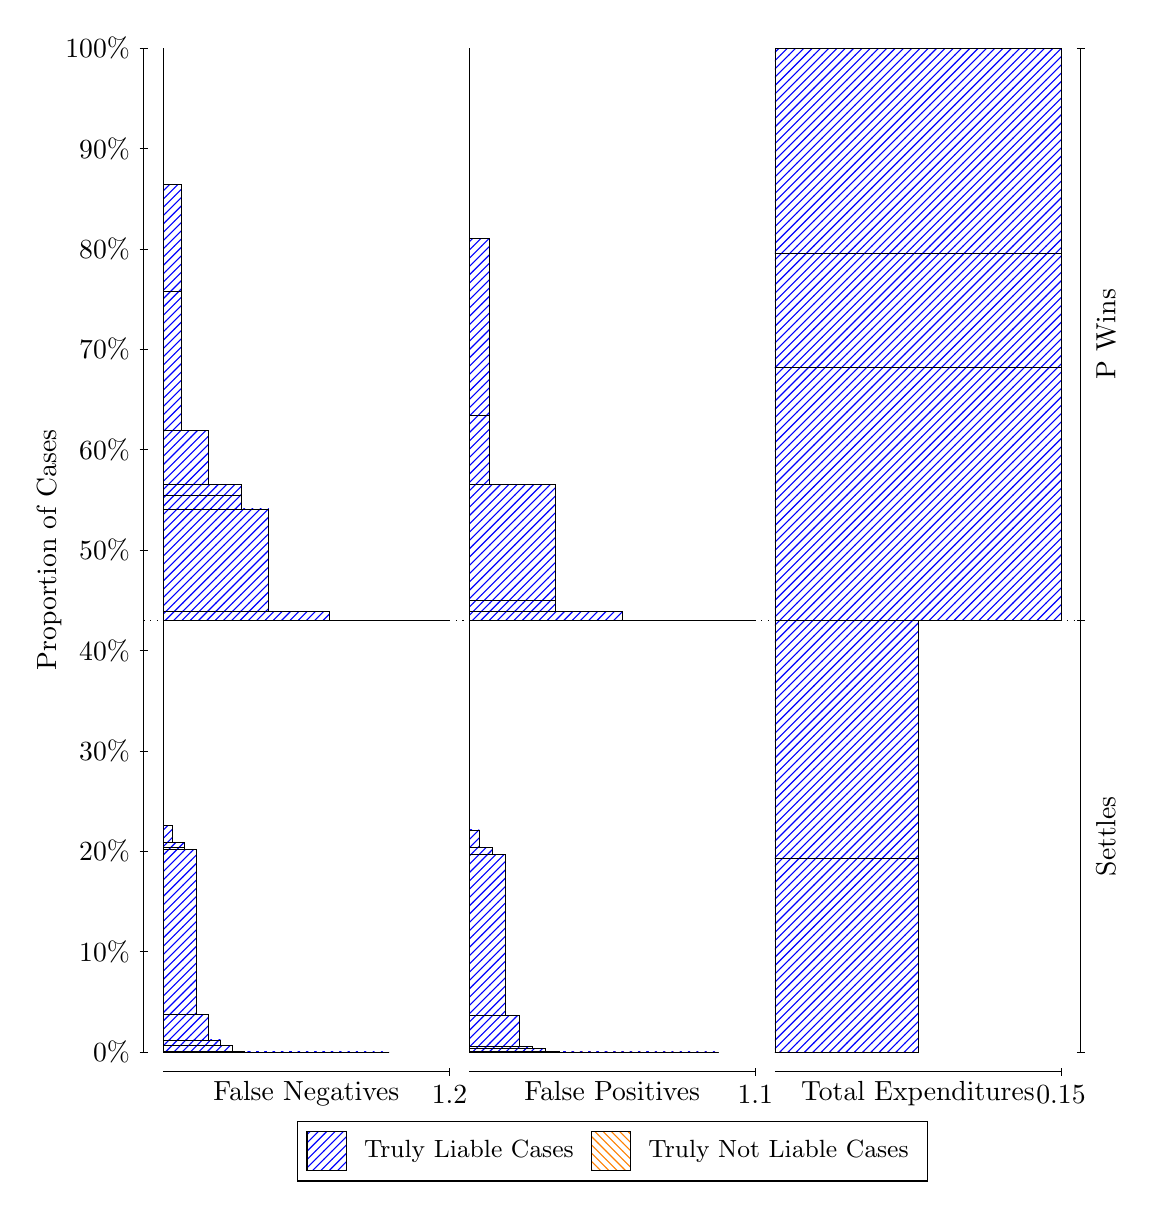
\begin{tikzpicture}
\draw[black, very thin] (1.5,1.75) -- (1.5,14.5);
\node[rotate=90, anchor=center] at (0.3, 8.125) {Proportion of Cases};
\draw[black, very thin] (1.45,1.75) -- (1.55,1.75);
\node[anchor=east] at (1.45, 1.75) {0\%};
\draw[black, very thin] (1.45,3.025) -- (1.55,3.025);
\node[anchor=east] at (1.45, 3.025) {10\%};
\draw[black, very thin] (1.45,4.3) -- (1.55,4.3);
\node[anchor=east] at (1.45, 4.3) {20\%};
\draw[black, very thin] (1.45,5.575) -- (1.55,5.575);
\node[anchor=east] at (1.45, 5.575) {30\%};
\draw[black, very thin] (1.45,6.85) -- (1.55,6.85);
\node[anchor=east] at (1.45, 6.85) {40\%};
\draw[black, very thin] (1.45,8.125) -- (1.55,8.125);
\node[anchor=east] at (1.45, 8.125) {50\%};
\draw[black, very thin] (1.45,9.4) -- (1.55,9.4);
\node[anchor=east] at (1.45, 9.4) {60\%};
\draw[black, very thin] (1.45,10.675) -- (1.55,10.675);
\node[anchor=east] at (1.45, 10.675) {70\%};
\draw[black, very thin] (1.45,11.95) -- (1.55,11.95);
\node[anchor=east] at (1.45, 11.95) {80\%};
\draw[black, very thin] (1.45,13.225) -- (1.55,13.225);
\node[anchor=east] at (1.45, 13.225) {90\%};
\draw[black, very thin] (1.45,14.5) -- (1.55,14.5);
\node[anchor=east] at (1.45, 14.5) {100\%};

\draw[black, very thin] (13.4,1.75) -- (13.4,14.5);
\draw[black, very thin] (13.35,1.75) -- (13.45,1.75);
\node[anchor=west] at (13.35, 1.75) {};
\draw[black, very thin] (13.35,7.2302) -- (13.45,7.2302);
\node[anchor=west] at (13.35, 7.2302) {};
\draw[black, very thin] (13.35,14.5) -- (13.45,14.5);
\node[anchor=west] at (13.35, 14.5) {};

\draw[black, very thin, pattern color=blue, pattern=north east lines] (1.75,1.75) rectangle (4.6184,1.75);
\draw[black, very thin, pattern color=blue, pattern=north east lines] (1.75,1.75) rectangle (4.3125,1.75);
\draw[black, very thin, pattern color=blue, pattern=north east lines] (1.75,1.75) rectangle (4.0065,1.75);
\draw[black, very thin, pattern color=blue, pattern=north east lines] (1.75,1.75) rectangle (3.8535,1.75);
\draw[black, very thin, pattern color=blue, pattern=north east lines] (1.75,1.75) rectangle (3.7005,1.75);
\draw[black, very thin, pattern color=blue, pattern=north east lines] (1.75,1.75) rectangle (3.5475,1.75);
\draw[black, very thin, pattern color=blue, pattern=north east lines] (1.75,1.75) rectangle (3.3946,1.7502);
\draw[black, very thin, pattern color=blue, pattern=north east lines] (1.75,1.7502) rectangle (3.2416,1.7503);
\draw[black, very thin, pattern color=blue, pattern=north east lines] (1.75,1.7503) rectangle (3.0886,1.7509);
\draw[black, very thin, pattern color=blue, pattern=north east lines] (1.75,1.7509) rectangle (2.9356,1.7515);
\draw[black, very thin, pattern color=blue, pattern=north east lines] (1.75,1.7515) rectangle (2.7826,1.7545);
\draw[black, very thin, pattern color=blue, pattern=north east lines] (1.75,1.7545) rectangle (2.6296,1.8381);
\draw[black, very thin, pattern color=blue, pattern=north east lines] (1.75,1.8381) rectangle (2.4767,1.9024);
\draw[black, very thin, pattern color=blue, pattern=north east lines] (1.75,1.9024) rectangle (2.3237,2.2265);
\draw[black, very thin, pattern color=blue, pattern=north east lines] (1.75,2.2265) rectangle (2.1707,4.3254);
\draw[black, very thin, pattern color=blue, pattern=north east lines] (1.75,4.3254) rectangle (2.0177,4.3439);
\draw[black, very thin, pattern color=blue, pattern=north east lines] (1.75,4.3439) rectangle (2.0177,4.4099);
\draw[black, very thin, pattern color=blue, pattern=north east lines] (1.75,4.4099) rectangle (1.8647,4.6285);
\draw[black, very thin, pattern color=orange, pattern=north west lines] (1.75,4.6285) rectangle (1.75,4.6285);
\draw[black, very thin, pattern color=blue, pattern=north east lines] (1.75,4.6285) rectangle (1.75,7.2302);
\draw[black, very thin, pattern color=blue, pattern=north east lines] (1.75,7.2302) rectangle (5.3833,7.2302);
\draw[black, very thin, pattern color=blue, pattern=north east lines] (1.75,7.2302) rectangle (4.6184,7.2314);
\draw[black, very thin, pattern color=blue, pattern=north east lines] (1.75,7.2314) rectangle (4.2742,7.2314);
\draw[black, very thin, pattern color=blue, pattern=north east lines] (1.75,7.2314) rectangle (3.8535,7.3426);
\draw[black, very thin, pattern color=blue, pattern=north east lines] (1.75,7.3426) rectangle (3.5093,7.3427);
\draw[black, very thin, pattern color=blue, pattern=north east lines] (1.75,7.3427) rectangle (3.0886,8.6477);
\draw[black, very thin, pattern color=blue, pattern=north east lines] (1.75,8.6477) rectangle (2.7444,8.8146);
\draw[black, very thin, pattern color=blue, pattern=north east lines] (1.75,8.8146) rectangle (2.7444,8.9623);
\draw[black, very thin, pattern color=blue, pattern=north east lines] (1.75,8.9623) rectangle (2.3237,9.6487);
\draw[black, very thin, pattern color=blue, pattern=north east lines] (1.75,9.6487) rectangle (1.9795,11.406);
\draw[black, very thin, pattern color=blue, pattern=north east lines] (1.75,11.406) rectangle (1.9795,12.769);
\draw[black, very thin, pattern color=orange, pattern=north west lines] (1.75,12.769) rectangle (1.75,12.769);
\draw[black, very thin, pattern color=blue, pattern=north east lines] (1.75,12.769) rectangle (1.75,14.5);
\draw[black, very thin, pattern color=orange, pattern=north west lines] (5.6333,1.75) rectangle (8.8019,1.75);
\draw[black, very thin, pattern color=blue, pattern=north east lines] (5.6333,1.75) rectangle (8.8019,1.75);
\draw[black, very thin, pattern color=orange, pattern=north west lines] (5.6333,1.75) rectangle (8.126,1.75);
\draw[black, very thin, pattern color=blue, pattern=north east lines] (5.6333,1.75) rectangle (8.126,1.75);
\draw[black, very thin, pattern color=blue, pattern=north east lines] (5.6333,1.75) rectangle (7.957,1.75);
\draw[black, very thin, pattern color=orange, pattern=north west lines] (5.6333,1.75) rectangle (7.788,1.75);
\draw[black, very thin, pattern color=blue, pattern=north east lines] (5.6333,1.75) rectangle (7.788,1.75);
\draw[black, very thin, pattern color=orange, pattern=north west lines] (5.6333,1.75) rectangle (7.45,1.75);
\draw[black, very thin, pattern color=blue, pattern=north east lines] (5.6333,1.75) rectangle (7.45,1.7501);
\draw[black, very thin, pattern color=blue, pattern=north east lines] (5.6333,1.7501) rectangle (7.281,1.7501);
\draw[black, very thin, pattern color=orange, pattern=north west lines] (5.6333,1.7501) rectangle (7.112,1.7501);
\draw[black, very thin, pattern color=blue, pattern=north east lines] (5.6333,1.7501) rectangle (7.112,1.7524);
\draw[black, very thin, pattern color=blue, pattern=north east lines] (5.6333,1.7524) rectangle (6.943,1.7524);
\draw[black, very thin, pattern color=orange, pattern=north west lines] (5.6333,1.7524) rectangle (6.774,1.7524);
\draw[black, very thin, pattern color=blue, pattern=north east lines] (5.6333,1.7524) rectangle (6.774,1.7544);
\draw[black, very thin, pattern color=blue, pattern=north east lines] (5.6333,1.7544) rectangle (6.605,1.7942);
\draw[black, very thin, pattern color=orange, pattern=north west lines] (5.6333,1.7942) rectangle (6.436,1.7942);
\draw[black, very thin, pattern color=blue, pattern=north east lines] (5.6333,1.7942) rectangle (6.436,1.8164);
\draw[black, very thin, pattern color=blue, pattern=north east lines] (5.6333,1.8164) rectangle (6.436,1.8175);
\draw[black, very thin, pattern color=blue, pattern=north east lines] (5.6333,1.8175) rectangle (6.2671,2.2145);
\draw[black, very thin, pattern color=orange, pattern=north west lines] (5.6333,2.2145) rectangle (6.0981,2.2145);
\draw[black, very thin, pattern color=blue, pattern=north east lines] (5.6333,2.2145) rectangle (6.0981,4.2608);
\draw[black, very thin, pattern color=blue, pattern=north east lines] (5.6333,4.2608) rectangle (6.0981,4.2609);
\draw[black, very thin, pattern color=blue, pattern=north east lines] (5.6333,4.2609) rectangle (5.9291,4.3518);
\draw[black, very thin, pattern color=blue, pattern=north east lines] (5.6333,4.3518) rectangle (5.7601,4.5703);
\draw[black, very thin, pattern color=blue, pattern=north east lines] (5.6333,4.5703) rectangle (5.6333,7.2302);
\draw[black, very thin, pattern color=orange, pattern=north west lines] (5.6333,7.2302) rectangle (9.2667,7.2302);
\draw[black, very thin, pattern color=blue, pattern=north east lines] (5.6333,7.2302) rectangle (9.2667,7.2302);
\draw[black, very thin, pattern color=orange, pattern=north west lines] (5.6333,7.2302) rectangle (8.4217,7.2302);
\draw[black, very thin, pattern color=blue, pattern=north east lines] (5.6333,7.2302) rectangle (8.4217,7.2314);
\draw[black, very thin, pattern color=orange, pattern=north west lines] (5.6333,7.2314) rectangle (7.5767,7.2314);
\draw[black, very thin, pattern color=blue, pattern=north east lines] (5.6333,7.2314) rectangle (7.5767,7.3416);
\draw[black, very thin, pattern color=orange, pattern=north west lines] (5.6333,7.3416) rectangle (7.1965,7.3416);
\draw[black, very thin, pattern color=blue, pattern=north east lines] (5.6333,7.3416) rectangle (7.1965,7.3416);
\draw[black, very thin, pattern color=orange, pattern=north west lines] (5.6333,7.3416) rectangle (6.7318,7.3416);
\draw[black, very thin, pattern color=blue, pattern=north east lines] (5.6333,7.3416) rectangle (6.7318,7.4877);
\draw[black, very thin, pattern color=blue, pattern=north east lines] (5.6333,7.4877) rectangle (6.7318,8.9577);
\draw[black, very thin, pattern color=orange, pattern=north west lines] (5.6333,8.9577) rectangle (6.3516,8.9577);
\draw[black, very thin, pattern color=blue, pattern=north east lines] (5.6333,8.9577) rectangle (6.3516,8.9608);
\draw[black, very thin, pattern color=blue, pattern=north east lines] (5.6333,8.9608) rectangle (5.8868,9.8387);
\draw[black, very thin, pattern color=blue, pattern=north east lines] (5.6333,9.8387) rectangle (5.8868,12.082);
\draw[black, very thin, pattern color=orange, pattern=north west lines] (5.6333,12.082) rectangle (5.6333,12.082);
\draw[black, very thin, pattern color=blue, pattern=north east lines] (5.6333,12.082) rectangle (5.6333,14.5);
\draw[black, very thin, pattern color=orange, pattern=north west lines] (9.5167,1.75) rectangle (11.333,1.75);
\draw[black, very thin, pattern color=blue, pattern=north east lines] (9.5167,1.75) rectangle (11.333,4.2111);
\draw[black, very thin, pattern color=orange, pattern=north west lines] (9.5167,4.2111) rectangle (11.333,4.2111);
\draw[black, very thin, pattern color=blue, pattern=north east lines] (9.5167,4.2111) rectangle (11.333,7.2302);
\draw[black, very thin, pattern color=orange, pattern=north west lines] (9.5167,7.2302) rectangle (13.15,7.2302);
\draw[black, very thin, pattern color=blue, pattern=north east lines] (9.5167,7.2302) rectangle (13.15,10.449);
\draw[black, very thin, pattern color=orange, pattern=north west lines] (9.5167,10.449) rectangle (13.15,10.449);
\draw[black, very thin, pattern color=blue, pattern=north east lines] (9.5167,10.449) rectangle (13.15,11.893);
\draw[black, very thin, pattern color=orange, pattern=north west lines] (9.5167,11.893) rectangle (13.15,11.893);
\draw[black, very thin, pattern color=blue, pattern=north east lines] (9.5167,11.893) rectangle (13.15,14.5);
\draw[black, dotted] (1.5,7.2302) -- (13.4,7.2302);
\draw[black, very thin] (1.75,1.5) -- (5.3833,1.5);
\node[anchor=north] at (3.5667, 1.5) {False Negatives};
\draw[black, very thin] (5.3833,1.45) -- (5.3833,1.55);
\node[anchor=north] at (5.3833, 1.45) {1.2};

\draw[black, very thin] (5.6333,1.5) -- (9.2667,1.5);
\node[anchor=north] at (7.45, 1.5) {False Positives};
\draw[black, very thin] (9.2667,1.45) -- (9.2667,1.55);
\node[anchor=north] at (9.2667, 1.45) {1.1};

\draw[black, very thin] (9.5167,1.5) -- (13.15,1.5);
\node[anchor=north] at (11.333, 1.5) {Total Expenditures};
\draw[black, very thin] (13.15,1.45) -- (13.15,1.55);
\node[anchor=north] at (13.15, 1.45) {0.15};

\node[black, centered, rotate=90] at (13.72, 4.4901) {Settles};
\node[black, centered, rotate=90] at (13.72, 10.865) {P Wins};

\draw (7.449999999999999,1.5) node[draw=none] (baseCoordinate) {};
\begin{scope}[align=center]
        \matrix[scale=0.5, draw=black, below=0.5cm of baseCoordinate, nodes={draw}, column sep=0.1cm]{
            \node[rectangle, draw, minimum width=0.5cm, minimum height=0.5cm, pattern=north east lines, pattern color=blue] {}; &
            \node[draw=none, font=\small] (B) {Truly Liable Cases}; &
            \node[rectangle, draw, minimum width=0.5cm, minimum height=0.5cm, pattern=north west lines, pattern color=orange] {}; &
            \node[draw=none, font=\small] (B) {Truly Not Liable Cases}; \\
            };
\end{scope}

\end{tikzpicture}
\end{document}